\documentclass[tikz,border=3mm]{standalone}
\usepackage{pgfplots}
\pgfplotsset{compat=1.16}
\begin{document}
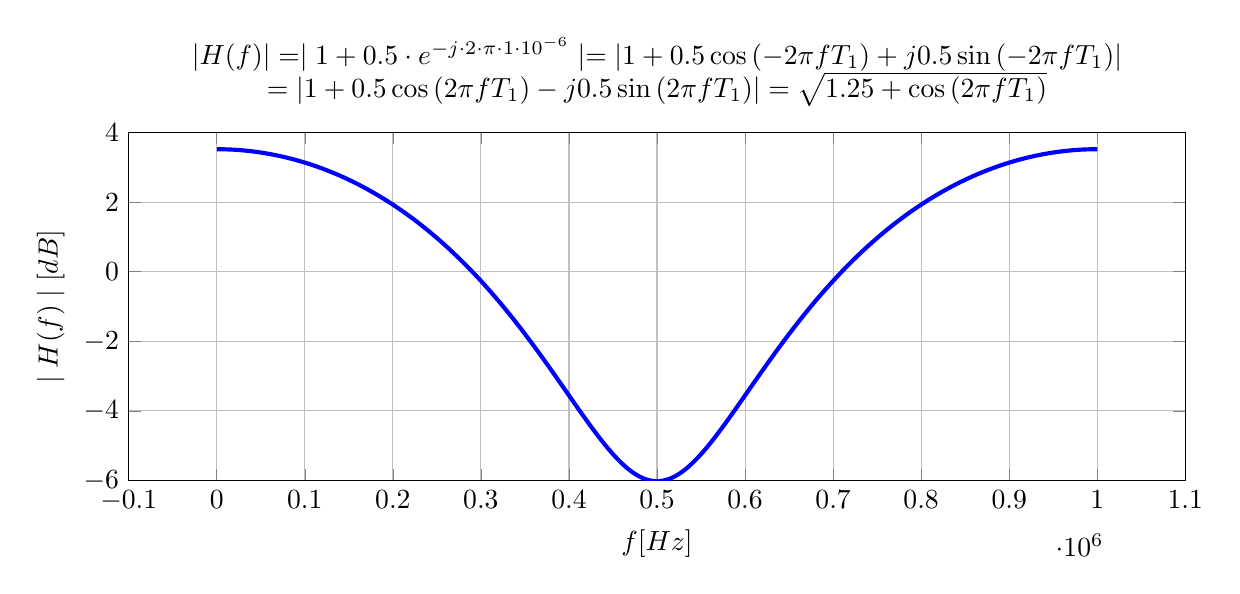
\begin{tikzpicture}
\begin{axis}[trig format plots=rad,
     width=15.0cm,
   height=6cm,
   grid=both,
   align =center,
   ymin=-6, ymax=4,
title={$
|H(f)| = \mid 1+ 0.5\cdot e^{-j\cdot2\cdot \pi\cdot 1\cdot10^{-6}} \mid =\left|1+0.5 \cos \left(-2 \pi f T_1\right)+j 0.5 \sin \left(-2 \pi f T_1\right)\right| $\\$
 =\left|1+0.5 \cos \left(2 \pi f T_1\right)-j 0.5 \sin \left(2 \pi f T_1\right)\right|=\sqrt{1.25+\cos \left(2 \pi f T_1\right)}$},
xlabel={$f[Hz]$},
ylabel={$\mid H(f)\mid [dB]$}]
\addplot[domain=0:10e5,color=blue,samples=1000,mark=none, line width = 1.5]{%
20*log10(sqrt(cos(2*pi*x*1e-6)+1.25))};
\end{axis}
\end{tikzpicture}
\end{document}